\message{ !name(main.tex)}%!TEX program = xelatex
\documentclass[a4paper,11pt]{article}%A4纸,正文为小四号字,对应12pt
%\usepackage[UTF8]{ctex}

%Add by DY.Feng
\usepackage[BoldFont,SlantFont,CJKchecksingle]{xeCJK}
\setCJKmainfont{SimSun}
\setCJKmonofont{SimSun}% 设置缺省中文字体

\usepackage{diagbox}

\usepackage{multido}


\usepackage{float}

\usepackage{algorithmic}

\usepackage{listings}
\usepackage{xcolor}
\lstset{escapechar=`,numbers=left
,basicstyle=\ttfamily
,backgroundcolor=\color[RGB]{245,245,244}
,keywordstyle=\bfseries\color[RGB]{130,0,0},identifierstyle=\bfseries\color[RGB]{0,0,130},numberstyle=\color[RGB]{41,41,255},commentstyle=\it\color[RGB]{130,130,130},stringstyle=\rmfamily\slshape\color[RGB]{255,0,0},showstringspaces=false,tabsize=4,texcl=true,frame=shadowbox,breaklines=true,float}

%设置引用
\usepackage[square]{natbib}
\bibliographystyle{GBT7714-2005NLang-UTF8} 

\setcitestyle{super}



%End

\usepackage{gzhubylw}
\begin{document}

\message{ !name(chapter03.tex) !offset(-39) }
%!TEX program = XeLaTeX
%!TeX root =main.tex
%请在花括号内输入本章标题,然后换行,输入本章内容。
\section{银行验证码分析}
我们收集了大陆5间银行的验证码进行识别,以1000个验证码为单位进行测试。

\begin{tabular}{|*{3}{c|}}
\hline
银行 & 验证码样本 & 识别率\% \\\hline
中国工商银行ICBC &   \includegraphics{./paper_images/icbc/1.eps} & 97.2
\\\hline 
招商银行CMB & \includegraphics{./paper_images/cmb/1.eps} & 98.6 \\\hline
%中国建设银行CCB
中国农业银行ABC & \includegraphics{./paper_images/abc/1.eps} & 82.1 \\\hline
中国光大银行CEB & \includegraphics{m./paper_images/ceb/1.eps} & 93.4 \\\hline
交通银行BCM &  \includegraphics{./paper_images/bcm/1.eps} & 80.2 \\

\hline
\end{tabular}

我们发现BCM和ABC的验证码识别率比较低,其原因是预处理过后的验证码有干扰
条的粘连,导致误识。而工商银行的背景看上去很复杂,其实使用本文第二章的
方法,改变图片的对比度,就能很好的提取出前景字符。

\subsection{对验证码改进的建议}

通过上面的试验,我们分析出到现有验证码的缺陷,对此我们给出一下建议
,一个比较牢固的字符验证码应该具有以下的特点:

\begin{itemize}
\item 字符要有比较高的粘连度。
\item 字符要有比较扭曲的变形,虽然字符变形已经可以用形状上下文描述子解
  决。
\item 干扰条的颜色要跟字符的颜色相似,以防止使用改变对比度的方法剔除干
  扰条。
\item 验证码的背景要跟要识别的字符颜色相似或者重合,否则多么复杂的背景
  也能很容易剔除。使用渐变颜色达到人眼辨别的最低要求。
\end{itemize}


\message{ !name(main.tex) !offset(-11) }

\end{document}